\ifx \globalmark \undefined %% This is default.
	\documentclass[twoside,openright,11pt,a4paper]{report}

%\compiler avec xelatex
%\usepackage[applemac]{inputenc}
\usepackage[T1]{fontenc}
\usepackage[utf8]{inputenc} %latin1 est possible
%\usepackage[latin1]{inputenc} %latin1 est possible
\usepackage[UKenglish]{babel}
\usepackage{lettrine}

%\usepackage[text={13cm,20cm},centering]{geometry}
\usepackage [squaren, Gray, mediumqspace]{SIunits}
\usepackage [top=2cm, bottom=2cm, left=2cm, right=2cm ]{geometry}

\renewcommand{\familydefault}{cmss}
\addto\captionsenglish{ \renewcommand\chaptername{Solutions of Chapte}}

\usepackage{graphicx}
\usepackage{amsmath}
\usepackage{amsfonts}
\usepackage{amssymb}
\usepackage{amsthm}
\usepackage{bm}
\usepackage{color}

\newcommand{\real}{\mathbb{R}}
\newcommand{\mb}{\mathbf}
\newcommand{\bos}{\boldsymbol}

\def \RR {I \! \! R}

\newcommand{\e}{\begin{equation}}  
\newcommand{\ee}{\end{equation}}
\newcommand{\eqn}{\begin{eqnarray}} 
\newcommand{\eeqn}{\end{eqnarray}} 
\newcommand{\eqnn}{\begin{eqnarray*}} 
\newcommand{\eeqnn}{\end{eqnarray*}} 

\newcommand{\bpm}{\begin{pmatrix}}
\newcommand{\epm}{\end{pmatrix}}

%\newcommand{\{\c c}}{\c c}

\newcommand{\bma}{\left(\begin{array}}
\newcommand{\ema}{\end{array}\right)} 
\newcommand{\hh}{\hspace{2mm}}
\newcommand{\hd}{\hspace{5mm}}
\newcommand{\hu}{\hspace{1cm}}
\newcommand{\vv}{\vspace{2mm}}
\newcommand{\vd}{\vspace{5mm}}
\newcommand{\vm}{\vspace{-2mm}}
\newcommand{\teq}{\triangleq}
%\newcommand{\qedb}{\,$\Box$}
\newcommand{\blanc}{$\left. \right.$}
\newcommand{\frts}[2]%
         {\frac{{\textstyle #1}}{{\textstyle #2}}}

\newcommand{\bindex}[3]%
{
\renewcommand{\arraystretch}{0.5}
\begin{array}[t]{c}
#1\\
{\scriptstyle #2}\\
{\scriptstyle #3}
\end{array}
\renewcommand{\arraystretch}{1}
}

\theoremstyle{definition}
\newtheorem{exemple}{{\bf Exemple}}[chapter]
\newtheorem{theoreme}[exemple]{{\bf Th{é}or{è}me}}
\newtheorem{propriete}[exemple]{{\bf Propri{é}t{é}}}
\newtheorem{definition}[exemple]{{\bf D{é}finition}}
\newtheorem{remarque}[exemple]{{\bf Remarque}}
\newtheorem{remarques}[exemple]{{\bf Remarques}}
\newtheorem{lemme}[exemple]{{\bf Lemme}}
\newtheorem{hypothese}[exemple]{{\bf Hypoth{è}se}}
\newtheorem{exercice}{{\bf Exercice}}[chapter]

\newcommand{\xqedhere}[2]{%
 \rlap{\hbox to#1{\hfil\llap{\ensuremath{#2}}}}}

\newcommand{\xqed}[1]{%
 \leavevmode\unskip\penalty9999 \hbox{}\nobreak\hfill
 \quad\hbox{\ensuremath{#1}}}

\newcommand{\gf}{\fg\,\,}

\newcommand{\cata}[1] %
     {\renewcommand{\arraystretch}{0.5}
     \begin{array}[t]{c} \longrightarrow \\ {#1} \end{array}
     \renewcommand{\arraystretch}{1}}

\usepackage[isu]{caption}
%\usepackage[font=small,format=plain,labelfont=bf,up,textfont=it,up]{caption}
\setlength{\captionmargin}{60pt}

\newcommand{\cqfd}
{%
\mbox{}%
\nolinebreak%
\hfill%
\rule{2mm}{2mm}%
\medbreak%
\par%
}

\pagestyle{headings}

\renewcommand{\sectionmark}[1]{%
\markright{\thesection.\ #1}{}}

\renewcommand{\chaptermark}[1]{%
\markboth{\chaptername\ \thechapter.\ #1}{}}

\makeatletter 
\def\@seccntformat#1{\csname the#1\endcsname.\;} 
\makeatother

\title{ {\Huge {\textbf{Modélisation et analyse  \\ \vspace{4mm} des systèmes dynamiques }}} \\ \vspace{4cm} G. Bastin}

%\title{ {\Huge {\textbf{Modelisation et analyse  \\ \vspace{4mm} des systemes dynamiques }}} \\ \vspace{4cm} G. Bastin}


\date{\today}
	\begin{document} %% Crashes if put after (one of the many mysteries of LaTeX?).
\else 
	\documentclass{standalone}
	\begin{document}
\fi

\graphicspath{ {images/} }	

\setcounter{chapter}{4}
\chapter{Reaction systems}
\chaptermark{Reaction systems}\label{sysreac}	
	
\lettrine[lines=1]{\bf T}{}he reaction system concept applies for a dynamic systems class used in various engineering domains such as chemistry, biomedical, biotechnologies or ecology. Under a spatial homogeneity assumption, reaction systems dynamic is described by 
balance differential equations.

These equations are obtained from a combination of a {\em reaction network }
which encodes the reactions that are supposed to occur in the system with two basic physical phenomena: 
the {\em reactions kinetic } from one part and the {\em exchange dynamics } from the other part.
Those various elements describing reaction systems will be presented in the following sections, starting by reaction networks.

\section{Reaction networks}
A reaction system is characterized by a given number of {\em reactions} between chemical or biological components.
The number of components is finite and we denote those components using the following symbols:
\eqnn 
X_1, X_2, X_3,  \ldots , X_n.
\eeqnn 
The number of reactions is also a finite number $m$ and those reactions occur inside a geometrically well defined domain.
For example, a chemical reactor if it occurs between chemical components or an ecological niche between animal species.
The domain boundary is also well defined and split the system from the external world.

The easiest way to introduce the reaction network concept is to start with an example.

\begin{exemple} {\bf Chemical reaction}

The reaction mechanism between nitric oxide and hydrogen is described 
using the following reaction network which has $m=4$ reactions employing $n=6$ chemical components:
\eqn 
2X_1 &\longrightarrow& X_2 \label{oxnit1}\\ 
X_2 &\longrightarrow& 2X_1 \\ 
X_2 + X_3&\longrightarrow& X_4 + X_5 \\ 
X_3 + X_5 &\longrightarrow& 2X_6 \label{oxnit4}  
\eeqn 
The six components are : $X_1 = NO$, $X_2 = N_2O_2$, $X_3 = H_2$, $X_4 = N_2$,
$X_5 = H_2O_2$, $X_6 = H_2O$.   \qed
\end{exemple}

A reaction network is therefore a set of $m$ reactions in the following form:
\eqnn 
\sum_{i=1}^n\gamma_{ij}X_i \longrightarrow
\sum_{i=1}^n\delta_{ij}X_i  \hspace{5mm} j=1,\ldots,m \hspace{5mm}
\gamma_{ij} \geq 0 \hspace{5mm} \delta_{ij} \geq 0.
\eeqnn 
The coefficients $\gamma_{ij}$ and $\delta_{ij}$ are positive real numbers called {\em stoichiometric coefficients}.
They represent the nominal quantity for the component $X_i$ 
which is consumed or produced by the $j^{th}$ reaction.
For example, the fourth network reaction above means: 
one mole of $X_3$ combined to one mole of $X_5$ produces two moles of $X_6$. 

We introduce the following matrix notations :
\begin{equation*} \begin{split}
\Gamma &= [\gamma_{ij}] \hh \hh \mbox{matrix } n \times m \text{ with elements } \gamma_{ij} \\
\Delta &= [\delta_{ij}] \hh \hh \mbox{matrix } n \times m \text{ with elements } \delta_{ij}
\end{split} \end{equation*}
The {\em stoichiometric matrix} is defined as :
\begin{equation*} \begin{split}
C = \Delta - \Gamma.
\end{split} \end{equation*}
The matrix rank $p$ is called the {\em reaction network rank}.
It corresponds to the numbers of independent reactions.

As a convention, all reactions are denoted with an arrow from the left to the right.
In the example above, the {\em reversible} reaction $2X_1 \leftrightarrows X_2$ 
is encoded as two simple distinct reactions : 
\eqnn 
2X_1 &\longrightarrow& X_2 \\ X_2
&\longrightarrow& 2X_1 
\eeqnn

\subsection* {Reactants and products}

The {\em reactants} are the components $X_i$ 
which are written on the left hand side of the arrow with a coefficient $\gamma_{ij} > 0$.

The {\em products} are the components $X_i$ 
which are written on the right hand side of the arrow with a coefficient $\delta_{ij} > 0$. 

A component $X_i$ can either be a reactant in a reaction and a product in another or the same reaction.
This is the case of the component $X_5$ in the example 5.1.

A {\em terminal product} is a component produced by at least one reaction but which is a reactant of none reaction.

An {\em initial reactant} is a component consumed by at least one reaction but which is produced by no reaction.

As an example, in the reaction network (\ref{oxnit1}) - (\ref{oxnit4}),
we identify the following subsets : 

\begin{tabular}{ccc}
Reactants & : & $X_1, X_2, X_3, X_5$ \\
Products  & : & $X_1, X_2, X_4, X_5, X_6$ \\
Initial reactant & : & $X_3$ \\
Terminal products & : & $X_4, X_6$ \\
\end{tabular}

\subsection* {Catalysts et autocatalysts}

As we just explained, a given component can be on both sides of a reaction.
The component $X_2$ is an example in the following reaction :
\eqnn \gamma_1X_1 + \gamma_2X_2 \longrightarrow \delta_2X_2 + \delta_3X_3 \eeqnn 

If $\gamma_2 = \delta_2$ the component $X_2$ is a {\em catalyst}, in other words a component which is neither consumed nor produced but whose presence is required to perform the reaction.

If $\gamma_2 < \delta_2$, the component $X_2$ is an {\em autocatalyst},
a component which is a catalyst in its own production.

We also use an alternative representation for catalytic and autocatalytic reactions.
It consists in not writing the catalyst on the left side of the reaction
but indicating it under the arrow without coefficient 
and balancing it on the right side of the reaction with the coefficient $\delta_2 - \gamma_2$ :
\eqnn \gamma_1X_1  \cata{X_2} (\delta_2 - \gamma_2)X_2 + \delta_3X_3 \eeqnn 

Among the most typical autocatalytic reaction examples we can quote 
polymerization reactions or microbial growth reactions as described in the following example.

\begin{exemple} {\bf \em Alcoholic fermentation}

The alcoholic fermentation underlying mechanism can be described by the following reaction network :

 \eqnn X_1 + 2.33X_2 +
0.525X_3 &\cata{X_4}& 3.5X_4 + 2.5X_5 + 3.66X_6 \nonumber \\ X_1 +
0.054X_3 &\cata{X_4}& 0.36X_4 + 1.89X_5 + 0.14X_6 + 1.88X_7 \nonumber \\
1.61X_2 + 0.193X_3 + X_7 &\cata{X_4}& 1.32X_4 + 0.68X_5 + 2.12X_6
\nonumber \eeqnn 

The seven components are :
glucose $X_1$, 
oxygen $X_2$,
ammoniac $X_3$,
yeasts $X_4$, 
carbon dioxide $X_5$, 
water $X_6$,
ethanol $X_7$.  \qed
\end{exemple}

\section{Reaction systems state model}

The presence of each component inside the system can be quantified.
The component $X_i$ concentration denoted $x_i(t)$ corresponds to its amount in the system divided by the mixture volume.
The concentrations vector, which is also the model state vector, is denoted:
$$ x(t) \teq (x_1(t), x_2(t), \cdots , x_n(t))^T. $$

The reaction rates, also called {\em reaction kinetics}, describes the speed at which reactants are consumed and products are produced per volume unit in the system,
according to the reaction network.
A reaction rate $r_j$ is associated to each reaction of the network $(j = 1, \cdots , m)$.

The reaction rates depend on each component concentrations $x_i$, 
but they can eventually also be influenced by other system physico-chemical factors, such as temperature, catalysts or pressure.

We will here consider reactions depending only on state $x$.
The reaction kinetics vector is denoted:  
$$  r(x) \teq (r_1(x), r_2(x), \cdots , r_m(x))^T.  $$

Each function $r_j : \mathbb{R}_{+}^{n} \rightarrow \mathbb{R}_{+}$ has positive values and is defined on the positive orthant. 
A reaction cannot occurs unless all the reactants are presents in the system. 
In other words, the reaction rate is therefore null if one of the reactants is missing.
Mathematically, this condition can be stated as: 
\begin{hypothese} \label{cond}
\eqn 
&& \mbox{1) } r_j(x) \geq 0 \hspace{3mm} \forall j \hspace{3mm} \forall x \in \mathbb{R}_{+}, \label{cond1}\\ 
&& \mbox{2) }  r_j(x) = 0 \mbox{ si } x_i = 0  \mbox{ for a value of } i, 
\in I^{rj} \label{cond2} 
\eeqn
where $I^{rj}$ stands for the index of the reactants used in reaction $j$ set (including  catalysts).  \qed
\end{hypothese}


Based on the reaction network description and the reaction rates, we can easily check
that the quantitative balance of each component inside the system bounds can be written as:
$$ \dot x_i = \sum_{j = 1}^{m} (\delta_{ij} - \gamma_{ij})r_j(x(t)) + \frac{1}{V}(Q_{0i}(t) - Q_{i0}(t)). \label{contireac} $$

In this equation, the notations $\delta_{ij}$, $\gamma_{ij}$ (stoichiometric coefficients) and $r_j(x(t))$ (reaction rate) were defined earlier.
The notation $V$ stands for the volume (assumed constant) of the domain.
The notations $Q_{0i}(t)$ and $Q_{i0}(t)$ stand for the flows of the component $X_i$ through the domain boundary :
\begin{description}
\item $Q_{io}(t)$ is the flow going from the domain towards the outside,
\item $Q_{oi}(t)$ is the flow going from the outside towards the domain.
\end{description}

This continuity equation states that the variation, per time unit, of the component concentration $X_i$ comes from two distinct mechanisms:
\begin{itemize}
\item $\sum_{j = 1}^{m} (\delta_{ij} - \gamma_{ij})r_j(x(t))$ express the difference, per volume unit, 
between the product quantities sum and consumed quantities sum in the reaction where this component $X_i$ is a product or a reactant respectively;
\item $Q_{0i}(t) - Q_{i0}(t)$ express the difference between the incoming flow and the outgoing flow from the same component $X_i$ towards the domain boundary.
\end{itemize}

The system is said to be {\em closed} when $Q_{io}(t) =  Q_{oi}(t) = 0$ for all $i$ and for all $t$,
in other words, when there is no exchange with the outside.
In the opposite situation, the system is said {\em open}. 

A reaction system state modeling has three fundamental aspects.

First, the reaction network determines the number of state variables, the structure and the numerical values of the stoichiometric matrix coefficients.

Second, we might ask ourselves how to model reaction rates $r_j(x)$ according to the state variables $x_i$.
The modeling will be presented in the following section.

We will then model the incoming and outgoing flows according to the state and the input variables: 
\eqnn
Q_{0i}(x,u) \hspace{1cm} Q_{i0}(x,u)
\eeqnn
This modeling will be illustrated using various examples.

Reaction system dynamic is therefore represented by the following state model:
\eqn 
\dot x =  Cr(x) + q_{in}(x,u) - q_{out}(x,u) \label{sysrea} 
\eeqn
where the definition of vectors $q_{in}(x,u)$ and $q_{out}(x,u)$ is obvious.
This state model can then only be defined on the positive orthant.
We can easily show that, under the \ref{cond} assumption, the system (\ref{sysrea}) is a positive system with a compartments system structure.

For a closed system, vectors $q_{in}$ and $q_{out}$ are identically zeros
and the state model can be reduced to the equation: 
$$ \dot{x} = Cr(x). \label{sysreaferm} $$

\begin{hypothese} \label{princon} {\bf \em The preservation principle}
The stoichiometric matrix kernel contains a positive vector:
$$ \exists \hh \omega = (\omega_1, \ldots , \omega_n)^T \hh
\omega_i > 0 \hh i=1,\ldots,n \hh \mbox{ tel que } \omega \in \ker C^T. \xqedhere{2cm}{\qed} $$
\end{hypothese}

Under this assumption, we easily check that the quantity
$$ z = \sum_{i=1}^m \omega_i x_i = \omega^Tx $$
is a system invariant (\ref{sysreaferm}) (in other words, $z(t)$ is constant along system solutions).

$$ \dot z = \sum_{i=1}^n \omega_i \dot x_i = [\omega^TC]r(x) = 0 $$
and the quantity between brackets is indeed zero thanks to the assumption \ref{princon}.

This assumption is essential because it express the fact that, according to the reality,
a closed reaction system is a preservative system; the total quantity inside the system is a constant:
the produced quantities are equal to the consumed quantities (using appropriate normalization coefficients).
As Lavoisier said, \og rien ne se perd, rien ne se crée \fg.


\section{Reaction kinetics modeling}
If a reaction respects the {\em Law mass action}, a classical general expression, respecting the conditions (\ref{cond1}) - (\ref{cond2}), can be written:
$$ r_j(x) = k_j\prod_{i \in I^{rj}} x_i^{\nu_{ij}} $$
where $k_j$ is the {\em rate constant} of the  $j^{th}$ reaction. 
The mass action principle consists in expressing each reaction rate as being proportional to the product of the reactants concentrations in the reaction
(including catalysts), each concentration being set to the $\nu_{ij}$ positive power called {\em order} of the $j^{reaction}$s.

The mass action Law corresponds to the particular case where $\nu_{ij} = \gamma_{ij} \hh \forall (i,j)$, 
where the reaction orders match the reactants stoichiometric coefficients.

However, the mass action principle is often not enough to match the experimentally observed reaction rates.
We therefore have to generalize the model :
\eqnn r_j(x) =  k_j\prod_{i \in I^{rj}} \rho_{ij}(x_i) \eeqnn
where functions $\rho_{ij} :\mathbb{R}_{+} \rightarrow \mathbb{R}_{+}$ 
respect the following conditions: 
\eqnn && \rho_{ij}(x_i) \geq 0 \hh \hh \forall x_i \geq 0 \\ && \rho_{ij}(0) = 0 \eeqnn

Functions  $\rho_{ij}(x_i)$ are often monotonically increasing function, as shown in figure \ref{Fig:monocrois}. 
\begin{figure}[htbp] 
   \centering
   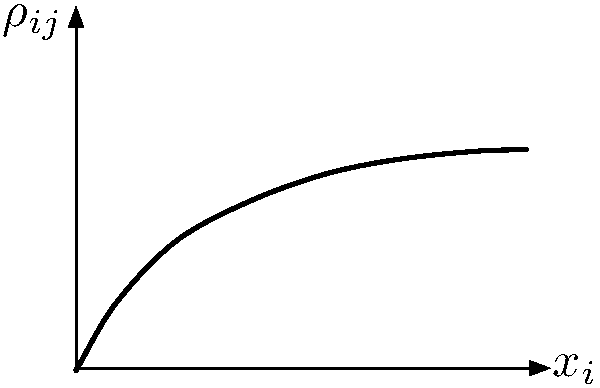
\includegraphics[height=4cm]{monocrois} 
   \caption{Monotonically increasing kinetic function}
   \label{Fig:monocrois}
\end{figure}
One of the most famous example is called the Michaelis-Menten kinetic and is represented by the function:
$$ \rho_{ij}(x_i) = \frac{x_i}{K_{ij} + x_i}. $$ 


\subsection*{Inhibitors and activators}
A reaction can be slowed down by a reaction product of any other component being in the reaction network.
Such an {\it inhibitor} effect is modeled by adding an additional multiplicative term in the kinetic model.
This term is a decreasing function of the inhibitor component concentration.
The two most frequent models are the following: 
\eqn 
&& \mbox{hyperbolic inhibition : } \rho_{ij}(x_i) = \frac {K_{ij}}{K_{ij} + x_i}, \label{inhibhyper} \\ && \mbox{exponential inhibition : } \rho_{ij}(x_i) = e^{-(K_{ij}x_i)}.
\label{inhibexpo} 
\eeqn

\begin{exemple}  Let consider the following reaction network:
\begin{equation} \begin{split} \label{exa}
X_1 + X_2 \; &\longrightarrow \; 2X_3, \\ 
2X_3 \; &\longrightarrow \; X_4. 
\end{split} \end{equation}
Suppose that kinetics respect the mass action law and that the first reaction is the most inhibited by the $X_4$ product of the second reaction, 
following an exponential law (\ref{inhibexpo}).
Both reaction kinetics will have the following form:
\begin{equation} \begin{split} \label{cin}
r_1(x) &= k_1x_1x_2e^{-(Kx_4)}, \\
r_2(x) &= k_2x_3^2. \xqedhere{6.2cm}{\qed}
\end{split} \end{equation}
\end{exemple}

A component in the reaction can also have a speed effect without being required to the reaction
(this component is nor a reactant nor a catalyst of the reaction).
Such {\it activator} effect is modeled by adding an additional multiplicative term in the kinetic model.
This term is an increasing function of the activator component concentration (which is non zero at start).

\section{Perfectly mixed reactors}

Perfectly mixed chemical or biological reactors form one of the most typical reaction system example.
Reactors consists in a vessel containing a liquid reaction medium which is permanently mixed by an appropriate agitation system and has an homogeneous composition.
The reactants can be provided to the reactor in liquid or gas state.
Reaction products are formed in the reaction system.
Some of these products can be easily gasified
and freely escape from the reactor under their gas state.
The reaction medium is removed from the reactor to collect the products.


\subsection {Réacteurs continus}

Un réacteur parfaitement mélangé fonctionne en {\em mode continu} lorsque les
débits d'alimentation et de soutirage sont ajustés de sorte que le volume $V$
du milieu réactionnel soit constant. On parle alors d'un réacteur continu
parfaitement mélangé (acronyme CSTR pour {\em
continuous stirred tank reactor}). Un exemple de réacteur de ce type est
représenté à la figure \ref{Fig:CSTR}. 
\begin{figure}[htbp] 
   \centering
   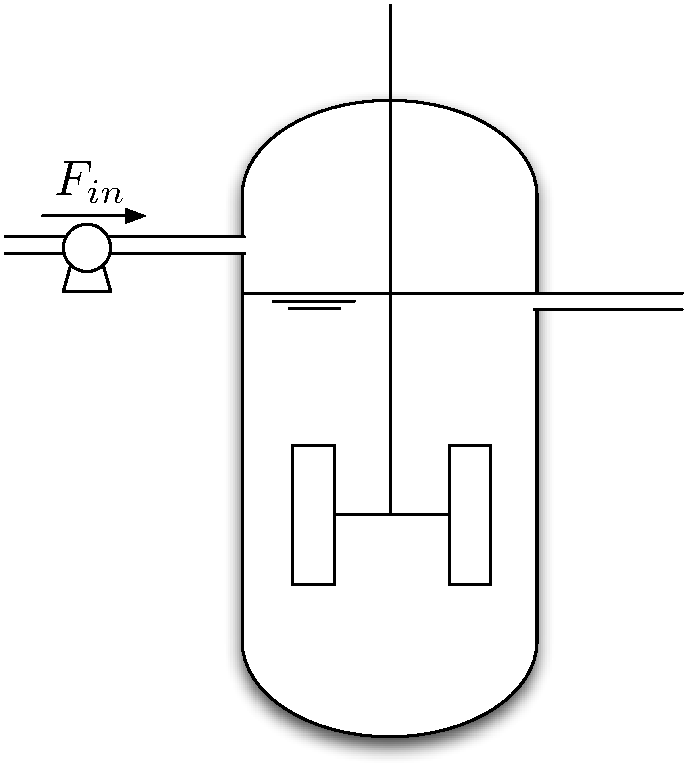
\includegraphics[height=6cm]{CSTR} 
   \caption{Réacteur continu parfaitement mélangé}
   \label{Fig:CSTR}
\end{figure}
Le réservoir est muni d'une canalisation d'alimentation et d'un dispositif de
trop-plein de manière à maintenir le volume constant.

On suppose que ce réacteur est le lieu d'un ensemble de $m$ réactions
impliquant $n$ espèces chimiques $X_1, X_2, \dots , X_n$. Les concentrations
des différentes espèces dans le milieu réactionnel sont notées  $x_i$. Les
diverses espèces sont fournies au réacteur en solution ou en suspension dans
le flux d'alimentation avec des concentrations notées $x_i^{in}$.
Le débit volumétrique d'alimentation est noté $F_{in}$. Avec ces notations et
définitions, les équations de bilan des différentes espèces dans le réacteur
s'écrivent sous la forme matricielle suivante~:
$$
\dot xV = Cr(x)V - F_{in}x + F_{in}x^{in}
$$
où $C$ est la matrice stoechiométrique du réseau réactionnel, $r(x)$ le vecteur
des vitesses de réactions, $x$ le vecteur des concentrations $x_i$ et $x^{in}$ le
vecteur des concentrations d'alimentation $x_i^{in}$.

En définissant la variable
d'entrée
$$ 
u \triangleq \frac{F_{in}}{V}
$$
qui est le débit d'alimentation par unité de volume, appelé aussi {\em taux de
dilution} (l'inverse du taux de dilution est le temps de séjour), on obtient le
modèle d'état d'un réacteur continu parfaitement mélangé~:
$$
\dot x = Cr(x) - ux + ux^{in}. \label{CSTR}
$$
On observe que ce modèle possède la structure (\ref{sysrea}) avec les
définitions suivantes~:
$$
q_{out}(x,u) = ux \hh \hh \hh q_{in}(x,u) = ux^{in}.
$$

\begin{exemple}{\blanc} \label{exempleCSTR}

Nous considérons un réacteur chimique parfaitement mélangé dans lequel
les deux réactions (\ref{exa}) se déroulent simultanément dans la
phase liquide avec les cinétiques (\ref{cin}).     Le réacteur est
alimenté par les deux réactifs initiaux $X_1$ et $X_2$ en solution avec des
concentrations d'alimentation
$x_1^{in}$ et $x_2^{in}$.

Le modèle d'état s'écrit
$$
\bma{c} \dot x_1 \\ \dot x_2 \\ \dot x_3 \\ \dot x_4 \ema =
\bma{cc} -1 & 0 \\ -1 & 0 \\ 2 & -2 \\ 0 & 1 \ema \bma{c}
k_1x_1x_2e^{-(Kx_4)} \\ k_2x_3^2 \ema 
 + u \bma{c} x_1^{in} -x_1 \\ x_2^{in} -x_2 \\ -x_3 \\ -x_4
\ema   
$$
où les variables d'état $x_1, x_2, x_3$ et $x_4$ représentent les
concentrations des différentes espèces dans le milieu réactionnel. \qed
\end{exemple}

\subsection{Réacteurs à volume variable}

Considérons maintenant le réacteur représenté à la figure \ref{Fig:CSTR2}. Il est
identique au précédent sauf que le trop-plein est remplacé par une canalisation
de soutirage dont le débit volumétrique $F_{out}$ est contrôlé par
une pompe. Dans le cas particulier où ce débit $F_{out}$ peut être nul par
intermittence (pas de soutirage), on dit que le réacteur fonctionne en mode
discontinu.
\begin{figure}[htbp] 
   \centering
   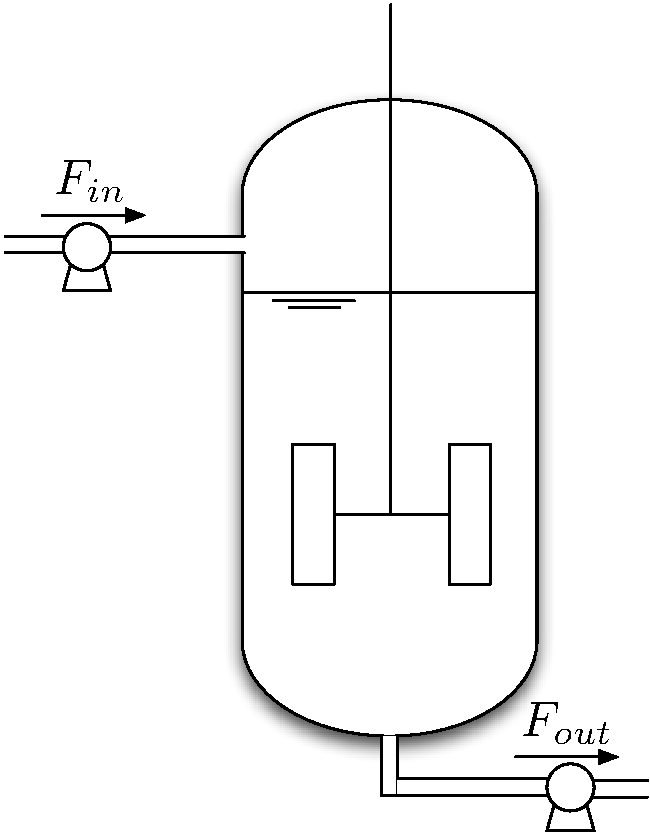
\includegraphics[height=6cm]{CSTR2} 
   \caption{Réacteur à volume variable}
   \label{Fig:CSTR2}
\end{figure}
L'équation matricielle de bilan massique des différentes espèces s'écrit
maintenant comme suit~:
$$
\frac{d}{dt} (xV) = Cr(x)V - F_{out}x + F_{in}x^{in}.
$$
Le volume du milieu réactionnel peut varier si les débits d'alimentation et de
soutirage sont différents. Les variations de volume sont décrites par l'équation de
bilan volumétrique~:
$$
\dot V = F_{in} -F_{out}.
$$
Si les deux débits volumétriques $F_{in}$ et $F_{out}$ sont
choisis comme variables d'entrée $u_1$ et $u_2$, on obtient le modèle d'état
suivant~: 
\begin{equation*} \begin{split}
\dot x &= Cr(x) + \frac{u_1}{x_{n+1}} (x^{in} - x), \\
\dot x_{n+1} &= u_1 - u_2,
\end{split} \end{equation*}
avec la variable d'état supplémentaire $x_{n+1}$ désignant le volume $V$.

Il est intéressant de choisir les débits par unité de volume $u_1 =
F_{in}/V$ et $u_2 = F_{out}/V$ comme variables d'entrée. Dans ce cas, le modèle
d'état s'écrit
\begin{equation*} \begin{split}
\dot x = Cr(x) + u_1(x^{in} - x), \\
\dot x_{n+1}= (u_1 - u_2)x_{n+1}.
\end{split} \end{equation*}
La première de ces deux équations décrit l'évolution de la
composition du réacteur. Elle est indépendante de $u_2$ et $x_{n+1}$ et elle est
identique à celle que nous avions obtenue pour un réacteur à volume constant
(\ref{CSTR}). 

\subsection{Réacteurs non-isothermes}

La vitesse d'une réaction chimique dépend aussi de la
température du milieu réactionnel. Jusqu'ici nous n'avons pas
pris cette dépendance en compte dans la modélisation : nous
avons implicitement supposé la température régulée à une
température parfaitement constante. En l'absence d'une telle
régulation, c'est la constante de vitesse qui dépend de la
température et la forme générale de la vitesse de la j-ième
réaction s'écrit
$$
r_j(x,T) = k_j(T)\rho_j(x)
$$
où $T$ désigne la température (en Kelvin) du milieu
réactionnel et la fonction $\rho_j(x)$ satisfait les conditions de
l'hypothèse (\ref{cond1})-(\ref{cond2}). La fonction $k_j(T)$ est
positive, bornée et $k_j(0) = 0$. Un exemple typique est donné
par la {\it loi d'Arrhenius} représentée à la figure
\ref{Fig:arrhenius}~: \eqnn
k_j(T) = k_{0j}exp(-\frac{E_j}{RT})
\eeqnn
\begin{figure}[htbp] 
   \centering
   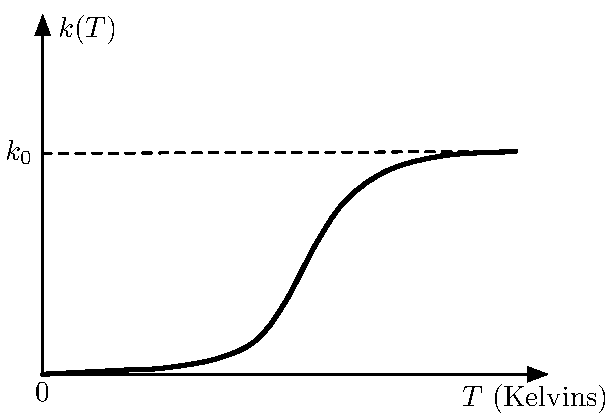
\includegraphics[width=8cm]{arrhenius} 
   \caption{Loi d'Arrhenius}
   \label{Fig:arrhenius}
\end{figure}
où $k_{0j}$ est une constante, $E_j$ l'énergie d'activation de la
réaction et $R$ la constante de Boltzmann. C'est une fonction
monotone croissante et bornée de la température. Dans
certaines applications (notamment en biotechnologie) la
fonction $k_j$ peut aussi être non monotone.

Le modèle d'état d'un réacteur non isotherme est obtenu en
ajoutant une équation de bilan énergétique aux équations de
bilan massique et volumique. A titre d'exemple, considérons un
réacteur continu muni d'un échangeur de chaleur.
L'équation de bilan énergétique s'écrit comme suit~:
$$
\delta c_p V\dot T = (\sum_{j=1}^{m}\Delta H_j r_j(x,T))V +
\delta c_p F_{in} (T_{in} - T) + Q
$$
où $\delta$ représente la densité du milieu réactionnel, $c_p$ la chaleur
spécifique, $\Delta H_j$ la chaleur de réaction, $T_{in}$ la
température du flux d'alimentation et $Q$ le flux de
chaleur échangé. Si on suppose que les paramètres $\delta$,
$c_p$ et $\Delta H_j$ sont constants, on obtient une équation
de bilan thermique~: 
$$ 
\dot T = \sum_{j=1}^{m} h_j r_j(x,T) +
d(T_{in} - T) + q
$$
où $h_j = \Delta H_j/c_p\delta V$ est la chaleur spécifique de
réaction, $d = F_{in}/V$ est le taux de dilution et $q =
Q/c_p \delta V$.

Les paramètres $h_j$ peuvent être positifs ou négatifs. Si
$h_j$ est négatif, la réaction en endothermique : elle
consomme de la chaleur qui est apportée dans le réacteur par
l'échangeur de chaleur. Si $h_j$ est positif, la réaction est
exothermique : elle génère de la chaleur dans le réacteur qui
doit être refroidi par l'échangeur de chaleur.

Le flux spécifique de chaleur échangée $q$ est lui même
fonction de la température $T$. Un modèle simple 
exprime que $q$ est proportionnel à la différence entre la
température du réacteur $T$ et la température d'entrée de
l'échangeur $T_w$~:
$$ q = e(T_w - T). $$
Dans ce cas, le modèle d'état global du réacteur s'écrit~:
\begin{equation*} \begin{split}
\dot x &= Cr(x) + d(x^{in} - x), \\
\dot x_{n+1} &= h^T r(x) + d(T_{in} - x_{n+1}) + e(T_w - x_{n+1}).
\end{split} \end{equation*}
avec la variable d'état supplémentaire $x_{n+1}$ désignant la
température $T$. Comme variables d'entrée, on peut choisir
par exemple le taux de dilution $d$ et le coefficient de
transfert thermique $e$ qui est proportionnel au débit de
l'échangeur de chaleur.

\section{Les systèmes écologiques} 

Le formalisme réactionnel et le
modèle d'état (\ref{sysrea}) conviennent aussi pour la description
d'une classe importante de systèmes écologiques (ou écosystèmes) dans
lesquels des populations d'organismes vivants (végétaux ou animaux) se
partagent un même habitat. 

Le modèle mathématique d'un écosystème se présente comme un cas
particulier de système réactionnel dans lequel~:
\begin{itemize}
\item le réseau réactionnel décrit les interactions entre espèces :
consommation de ressources inertes, pâturage sur des ressources
végétales, prédation, etc.  Les réactions sont nécessairement
autocatalytiques. 
\item les flux d'entrée représentent la fourniture de ressources au
système par des agents extérieurs et l'immigration de certaines espèces.
\item les flux de sortie représentent l'émigration des espèces vers
l'extérieur, la capture par des agents extérieurs (chasse, pêche, récolte,
cueillette, \dots) ou simplement la mortalité naturelle des espèces.
\end{itemize}

Nous commençons par un exemple simple.

\begin{exemple}{\bf \em Des algues dans la lagune}

Un nutriment organique provenant par exemple d'eaux ménagères
résiduaires ou de fertilisants agricoles est déversé dans une lagune. Une
population d'algues unicellulaires flottantes (phytoplancton) se développe
à la surface de l'eau en se nourrissant de ce nutriment. Cette situation peut
être schématisée par la réaction~:
\eqn
kY \longrightarrow X. \label{reacrois}
\eeqn
qui exprime que, dans le mécanisme de croissance des algues, le nutriment
$Y$ est transformé en matière vivante (ou biomasse) $X$ avec un
rendement $k^{-1}$. Comme tous les êtres vivants, les algues de la lagune
peuvent aussi mourir.

La lagune peut dès lors être considérée comme un vaste réacteur qui
transforme un réactif $Y$ (le nutriment) en un produit $X$ (la
biomasse). Le réacteur est alimenté par un flux entrant de réactif (le
nutriment déversé dans la lagune) tandis que la mortalité provoque un flux
sortant de produit. Sous une hypothèse
d'homogénéité spatiale, la dynamique de ce réacteur est décrite par
le modèle d'état
\begin{equation} \begin{split} \label{lagune}
\dot y &= -kr(x,y) + v, \\
\dot x &= r(x,y) - dx.
\end{split} \end{equation}
où $y$ représente la concentration en nutriment, $x$ la densité de la
population d'algues, $v$ le débit (par unité de volume) d'alimentation de la
lagune en nutriment, $dx$ la mortalité supposée proportionnelle à la
densité de population (le coefficient $d$ est le taux spécifique de
mortalité) et $r(x,y)$ la vitesse de réaction, c'est-à-dire ici la vitesse
de croissance des algues. \qed
\end{exemple}
D'un point de vue plus général, la réaction (\ref{reacrois}) peut
représenter la croissance d'une population quelconque d'organismes vivants
(végétaux ou animaux) $X$ qui, dans un habitat déterminé, consomme
une ressource alimentaire $Y$. Cette ressource alimentaire peut être de
la matière inerte (organique ou inorganique) comme dans l'exemple
ci-dessus. Elle peut aussi être une autre espèce vivante (végétale ou animale) : on parle
alors d'un modèle {\em proie - prédateur} dans lequel l'espèce ressource
$Y$ est la proie et l'espèce consommatrice $X$ est le prédateur.
D'évidence, cette réaction de croissance est autocatalytique puisque $X$
représente nécessairement une population d'êtres vivants autoreproducteurs~: 
\eqnn
kY \cata{X} X.
\eeqnn
Il est dès lors naturel de considérer que la vitesse de croissance est
proportionnelle à la densité de la population prédatrice et de représenter
la fonction $r(x,y)$ par un modèle de la forme~:
\eqnn
r(x,y) \teq \mu(x,y)x
\eeqnn
où la fonction $\mu(x,y)$ est appelée {\em vitesse spécifique de
croissance}. Cette fonction doit être définie de sorte que la vitesse de
réaction vérifie les conditions (\ref{cond1}) - (\ref{cond2}), c'est-à-dire~:
\begin{itemize}
\item $\mu(x,y)$ est une fonction positive définie sur l'orthant positif~:
\eqnn
\mu(x,y) \geq 0 \hh \hh \forall (x,y) \in \mathbb{R}_{+}^{2}.
\eeqnn
\item $\mu(x,0) = 0$ : il ne peut y avoir de croissance en l'absence de
ressource alimentaire.
\end{itemize}
La vitesse spécifique de croissance peut dépendre de nombreux facteurs
environnementaux. Deux effets non linéaires typiques sont l'effet de
{\em satiété} et l'effet de {\em surpopulation}.
\begin{description}
\item[Effet de satiété :] Lorsque la ressource alimentaire est rare, on
observe géné- ralement que la vitesse spécifique de croissance est une
fonction croissante de la quantité de ressource disponible. Il existe
cependant une limite physiologique à la vitesse de consommation
de la ressource et donc à la vitesse de croissance. Ceci se
modélise simplement en adoptant pour $\mu(x,y)$ une fonction
croissante saturée par rapport à $y$, telle que la vitesse de croissance
devient indépendante de $y$ au delà d'une concentration critique
$y_{c}$~: 
\eqnn
\frac{\partial \mu(x,y)}{\partial y} \geq 0, \hspace{1cm}
\mu(x,y) = \mu(x,y_{c}) \hh \hh \forall \hh y \geq y_{c}.
\eeqnn
\item[Effet de surpopulation :] Même quand la ressource alimentaire est
surabondante, la densité de la population est généralement limitée par
l'espace disponible. Ceci se modélise en imposant que la vitesse spécifique de
croissance $\mu(x,y)$ soit une fonction décroissante de la densité $x$
qui devient nulle quand la population atteint une valeur maximale $x_{m}$~:
 \eqnn
\frac{\partial \mu(x,y)}{\partial x} \leq 0, \hspace{1cm}
\mu(x,y) = 0 \hh \hh \forall \hh x \geq x_{m}.
\eeqnn
\end{description}

\begin{exemple}{\bf Le modèle de Contois.}

C'est un modèle classique de vitesse spécifique utilisé
pour décrire la croissance de populations de micro-organismes~:
\eqnn
\mu(x,y) = \frac{\mu_0 y}{y + Kx}.
\eeqnn
On observe que ce modèle est bien une fonction croissante bornée de $y$
(identique, à $x$ fixé, au modèle de Michaelis-Menten) et
décroissante (hyperbolique) de $x$. Cependant, les concentrations limites
de satiété $y_{c}$ et de surpopulation $x_{m}$ sont rejetées à l'infini.  \qed
\end{exemple}

\begin{exemple}{\bf Le modèle logistique}

Il est courant d'adopter pour la vitesse spécifique de croissance une
structure multiplicative de la forme~:
\eqnn
\mu(x,y) = \sigma(y)\phi(x).
\eeqnn
Cette structure permet de modéliser séparément les effets de satiété et
de surpopulation, par exemple de la manière suivante~:
\begin{equation*} \begin{split} \sigma(y) &= \left\{\begin{array}{ll}
\alpha y & \forall y \leq y_{c} \\ \alpha y_{c} & \forall y \geq y_{c} \end{array} \right.\\ \\
\phi(x) &= 
\left\{ \begin{array}{ll} (1 - \frac{x}{x_{m}}) & \forall x \leq x_{m} \\ 0  & \forall x \geq x_{m}
\end{array} \right.
\end{split} \end{equation*}
On observe que les fonctions $\sigma$ et $\phi$ sont linéaires et
saturées (voir figure  \ref{Fig:logistic}).
\begin{figure}[htbp] 
   \centering
   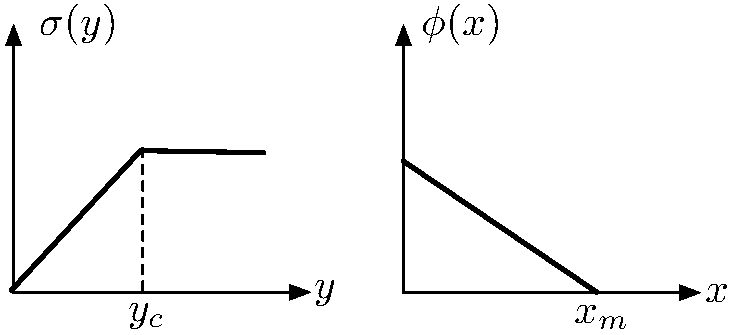
\includegraphics[height=5cm]{logistic} 
   \caption{Vitesse spécifique de croissance du modèle logistique}
   \label{Fig:logistic}
\end{figure}
Avec ces définitions, le modèle proie-prédateur
(\ref{lagune}) s'écrit, lorsque $y \leq y_{c}$ et $x \leq x_{m}$,
\begin{equation*} \begin{split}
\dot y &= -k\alpha xy(1 - \frac{x}{x_{m}}) + v, \\
\dot x &= \alpha xy(1 - \frac{x}{x_{m}}) - dx.
\end{split} \end{equation*}
Par contre, quand la ressource alimentaire est fournie au système en
quantité suffisante pour en maintenir la concentration au dessus de sa
valeur critique ($y(t) \geq y_{c} \hh \forall t$), alors la dynamique de
la population prédatrice devient {\em indépendante de la quantité de
ressource alimentaire disponible} et s'écrit simplement~:
\eqn
\dot x = \sigma_{c}x(1 - \frac{x}{x_{m}}) - dx  \label{logis}
\eeqn
où $\sigma_c = \alpha y_c$. La fonction $\phi(x) = (1 - x/x_{m})$ est généralement
dénommée {\em modèle logistique} dans la littérature. Par extension, le
modèle (\ref{logis}) est appelé modèle logistique de croissance d'une
population sur une ressource alimentaire non limitante.   \qed
\end{exemple}

Nous avons considéré jusqu'ici un modèle simple ne faisant intervenir que
deux espèces $X$ et $Y$. Cette description s'étend sans difficulté à
des écosystèmes plus complexes dans lesquels plusieurs espèces
biologiques, végétales ou animales, peuvent coexister et interagir au sein
d'un même habitat. Voici un exemple.

\begin{exemple} {\bf Un écosystème aquatique}

Un écosystème aquatique, comme tout système écologique naturel, est
géné-ralement caractérisé par la cohabitation de trois types
d'espèces biologiques : des espèces végétales, des espèces
animales herbivores et des espèces animales carnivores.  
\begin{figure}[htbp] 
   \centering
   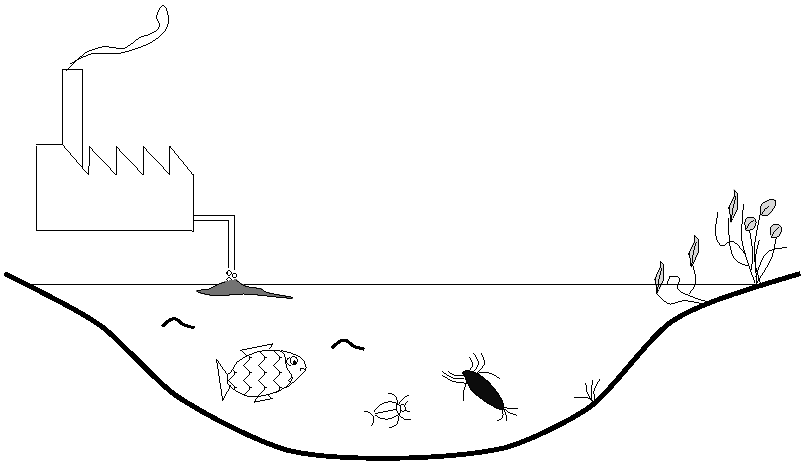
\includegraphics[height=5cm]{aquatic} 
   \caption{Ecosystème aquatique}
   \label{Fig:aquatic}
\end{figure}
A titre d'exemple, considérons un étang (voir figure
\ref{Fig:aquatic}) dans lequel est déversé un nutriment organique $X_1$.
Un population d'algues (phytoplancton) $X_2$
se développe par consommation de ce nutriment.  Une population de petits
crustacés herbivores $X_3$ p\^ature sur le phytoplancton qui constitue sa
ressource alimentaire principale. Une population de poissons carnivores $X_4$
assure son développement et sa subsistance par la consommation des
crustacés. La respiration animale consomme l'oxygène $X_5$ en solution
dans l'eau produit par la photosynthèse. Cette description est
schématisée par le réseau réactionnel suivant~:
\eqnn
c_1X_1 &\cata{X_2}& X_2 + c_4X_5, \\
c_2X_2 + c_5X_5 &\cata{X_3}& X_3, \\
c_3X_3 + c_6X_5 &\cata{X_4}& X_4. 
\eeqnn
Un modèle d'état du système est établi sous les hypothèses de
modélisation et avec les notations suivantes.
\begin{itemize}
\item Le nutriment organique est déversé avec un débit par unité de
volume $v$.
\item les trois espèces biologiques sont sujettes à une mortalité
naturelle. Les coefficients de mortalité sont notés $d_i, i = 2,3,4$.
\item Les poissons sont de plus l'objet d'une pêche dont l'intensité est
proportionnelle à la densité de la population. Le coefficient de
proportionnalité est noté $d_1$. 
\item La cinétique de croissance des
algues est décrite par le modèle logistique, avec une dépendance de
Michaelis Menten par rapport à la concentration en nutriment. 
\item Les deux
cinétiques de croissance des populations animales sont décrites par le
modèle de Contois avec une dépendance de Michaelis Menten par rapport
à la concentration en oxygène dissous. 
\end{itemize} 
Le modèle d'état de
cet écosystème aquatique s'écrit~: 
\begin{equation*} \begin{split}
\bma{c}  \dot x_1 \\ \dot x_2 \\
\dot x_3 \\ \dot x_4 \\ \dot x_5 \ema &= \bma{ccc} -c_1 & 0 & 0\\ 1 & -c_2
& 0 \\ 0 & 1 & -c_3 \\ 0 & 0 & 1 \\ c_4 & -c_5 & -c_6 \ema \bma{c}
\frac{{\textstyle \mu_1 x_1 x_2}}{{\textstyle x_1 + K_1}}(1 -
\frac{{\textstyle x_2}}{{\textstyle x_{2c}}}) \\ 
\\
\frac{{\textstyle \mu_2 x_2 x_3}}{{\textstyle x_2 + K_2x_3}}  \frac{{\textstyle
x_5}}{{\textstyle x_5 +K_4}} \\
\\
\frac{{\textstyle \mu_3 x_3 x_4}}{{\textstyle x_3 + K_3x_4}} \frac{{\textstyle
x_5}}{{\textstyle x_5 +K_5}}
\ema 
\\ & \\&- \bma{ccccc} 0 & 0 & 0 &
0 & 0 \\ 0 & d_2 & 0 & 0 & 0 \\0 & 0 & d_3 & 0 & 0  \\0 & 0 & 0 & d_1 + d_4 & 0
\\0 & 0 & 0 & 0 & 0
\ema \bma{c} x_1 \\  x_2 \\  x_3 \\  x_4 \\ x_5 \ema + \bma{c} v \\ 0  \\ 0 \\
0 \\ 0 \ema.    
\end{split} \end{equation*}
Les variables d'état
$x_2,x_3,x_4$ désignent les densités des trois populations biologiques
tandis que $x_1$ et $x_5$ désignent respectivement les concentrations en
nutriment et en oxygène dissous. \qed
\end{exemple}
 
\section{Exercices}

\begin{exercice}{\bf \em Un procédé chimique}

Une installation de génie chimique est représentée à la figure
\ref{Fig:genchim}. Une réaction réversible $A+B \leftrightarrow C$, obéissant
à la loi d'action des masses, se déroule dans le réacteur.
\begin{figure}[htbp] 
   \centering
   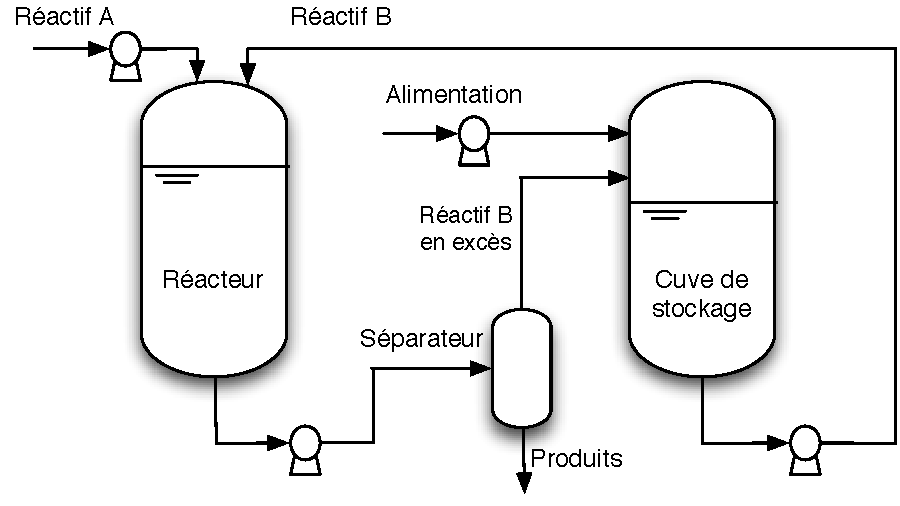
\includegraphics[height=6cm]{genchim} 
   \caption{Un procédé chimique}
   \label{Fig:genchim}
\end{figure}
 Le séparateur est
supposé opérer une séparation parfaite et instantanée des trois
espèces chimiques. Le réactif $B$ est recyclé via une cuve de
stockage. Le réactif $A$ et le produit $C$ sont soutirés du système.
Proposer un modèle d'état du système. \qed
\end{exercice}
\vv

\begin{exercice}{\bf \em Réacteur avec alimentations séparées}

Nous avons considéré dans ce chapitre que les différentes espèces qui alimentent un
réacteur sont fournies ensemble par une canalisation unique (voir par exemple la
figure \ref{Fig:CSTR}). Un tel dispositif peut avoir l'inconvénient de voir les
réactions débuter dans la canalisation d'amenée avant d'atteindre le réacteur. Cet
inconvénient est évité si les réactifs sont introduits dans le réacteur par des
canalisations séparées. Reconsidérons l'exemple \ref{exempleCSTR} avec des alimentations séparées pour
les deux réactifs $X_1$ et $X_2$ (voir figure \ref{Fig:CSTRsepar})~:
\begin{figure}[htbp] 
  \centering
   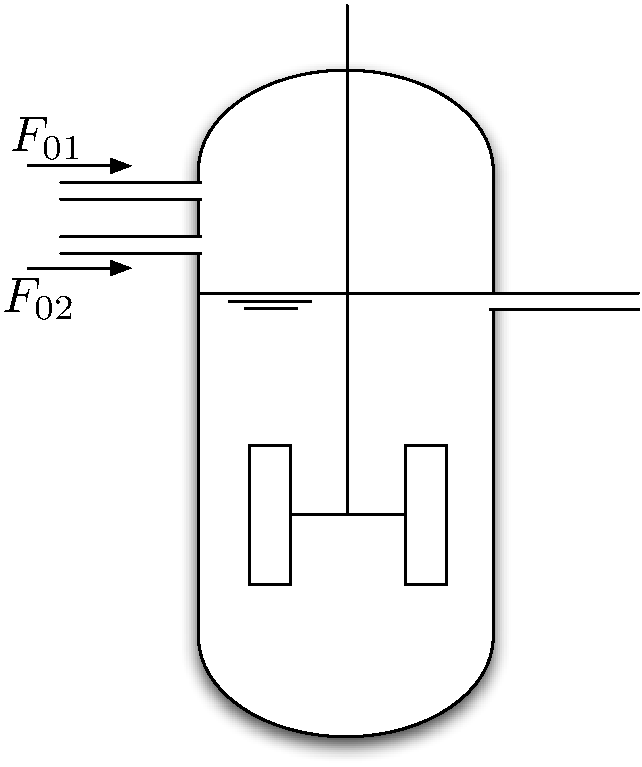
\includegraphics[height=6cm]{CSTRsepar} 
   \caption{Réacteur continu avec alimentations séparées}
   \label{Fig:CSTRsepar}
\end{figure}
\begin{enumerate}
\item Etablir un modèle d'état du système si les variables d'entrée sont les deux débits volumique d'alimentation $F_{01}$ et $F_{02}$.
\item Un cas particulier intéressant est celui ou le réacteur
est alimenté à débit volumique total constant ($F_{01} + F_{02} =$ constante).
Seule la composition de l'alimentation est variable. En pratique cela peut être
réalisé en ajustant complémentairement les deux débits $F_{01}$ et $F_{02}$
avec une vanne à quatre voies (voir figure \ref{Fig:vanne4voies}) de manière
que leur somme soit constante.  
\begin{figure}[htbp] 
   \centering
   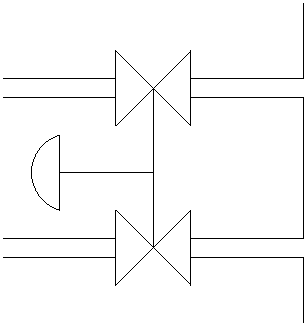
\includegraphics[height=4cm]{vanne4voies} 
   \caption{Alimentations séparées avec vanne à quatre voies}
   \label{Fig:vanne4voies}
\end{figure}
On choisit le débit $F_{01}$
comme unique variable d'entrée et on définit le taux de dilution constant $d =
(F_{01} + F_{02})/V$. Etablir le modèle d'état du système et montrer qu'il s'écrit sous la forme (\ref{sysrea}). \qed
\end{enumerate}
\end{exercice}
\vv

\newpage
\begin{exercice}{\bf \em Réactifs et produits gazeux}

Le modèle d'état (\ref{CSTR}) d'un réacteur continu parfaitement mélangé
peut être étendu au cas de réactifs ou de produits gazeux. Supposons tout
d'abord que le réacteur soit alimenté par un réactif $X$ sous forme gazeuse
(par exemple de l'oxygène) avec un débit massique $Q_{in}$ (voir figure
\ref{Fig:CSTRgaz}).
\begin{figure}[htbp] 
   \centering
   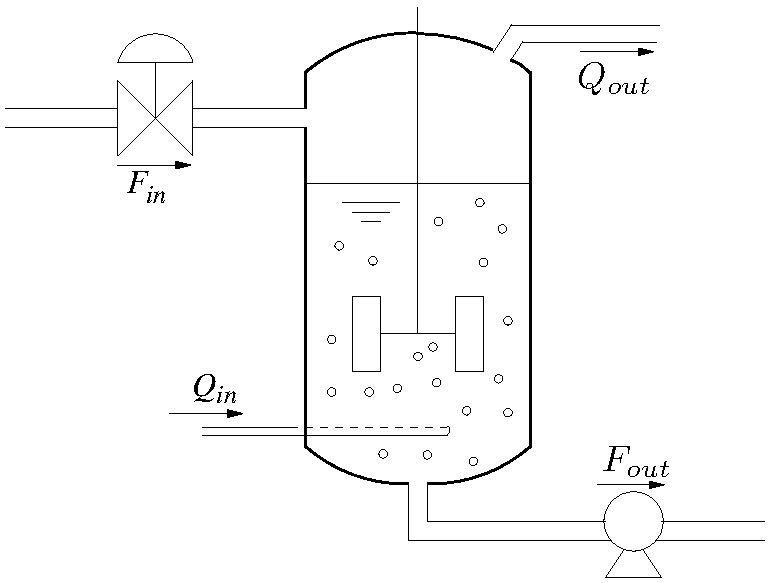
\includegraphics[height=6cm]{CSTRgaz} 
   \caption{Réacteur avec réactifs et produits gazeux}
   \label{Fig:CSTRgaz}
\end{figure}
Le réactif barbote dans le milieu liquide où il est partiellement dissous. L'excès de
réactif non-dissous s'échappe librement du réacteur sous forme gazeuse avec un
débit massique $Q_{out}$. La quantité de réactif mise en solution par unité
de temps est donc $Q_{in} - Q_{out}$. En se basant sur la loi de Henry et en
négligeant la dynamique du transfert gaz-liquide, on peut modéliser cette
quantité comme étant proportionnelle au débit gazeux d'alimentation d'une part
et au déficit de saturation d'autre part~:
\eqnn
Q_{in} - Q_{out} = aQ_{in}(x^{sat} - x)
\eeqnn
où $x$ désigne la concentration de l'espèce $X$ en solution et $x^{sat}$ la
concentration de saturation de cette même espèce dans la phase liquide.

Considérons maintenant qu'un produit de réaction $X$ (par exemple du $CO_2$)
formé en solution est gazéifiable. Il s'échappe du milieu réactionnel avec un débit
massique $Q_{out}$. Sous une hypothèse d'équilibre entre les phases liquide et
gazeuse, on peut considérer que ce débit est proportionnel à la concentration du
produit $X$	en solution dans le milieu réactionnel~:
\eqnn
Q_{out} = dx
\eeqnn
\begin{enumerate}
\item Comme dans l'exemple \ref{exempleCSTR}, considérons un réacteur
continu  dans lequel
 les deux réactions (\ref{exa})-(\ref{exb})
se déroulent simultanément dans la phase liquide avec les cinétiques
(\ref{cin}).  Cette fois, nous supposons cependant que le
réactif $X_2$ et le produit $X_4$ sont sous forme gazeuse. 
On demande d'établir le modèle d'état du système sous les hypothèses de modélisation suivantes~: 
\begin{itemize} 
\item Le réacteur est alimenté par le réactif initial $X_1$ en
solution avec un débit volumétrique $F_{in}$ et une
concentration d'alimentation $x_1^{in}$. 
\item Le réactif $X_2$ est injecté dans le réacteur sous forme gazeuse.
  La quantité de réactif $X_2$ mise en
solution par unité de temps est notée $aQ_{in}(x_2^{sat} - x_2)$.
\item Les produits $X_3$ et $X_4$ sont
formés en solution dans le milieu réactionnel. Le produit $X_4$ est
gazéifiable et s'échappe du réacteur avec un débit gazeux $dx_4$.
\end{itemize}
\item Si les variables d'entrée sont le débit volumétrique d'alimentation liquide par unité de
volume de milieu réactionnel $u_1 = F_{in}/V$ et le débit massique d'alimentation
gazeuse par unité de volume de milieu réactionnel $u_2 = Q_{in}/V$, montrer
que le modèle d'état possède la structure (\ref{sysrea}). \qed
\end{enumerate}
\end{exercice}
\vv

\begin{exercice}{\bf \em Une réacteur biochimique}

Un réacteur biochimique fonctionnant en mode CSTR met en jeu trois
espèces : une population bactérienne $X_1$, du glucose $X_2$,
et du lactose $X_3$.\\

La dynamique du réacteur est décrite par le modèle d'état suivant
($x_i$ désigne la concentration de l'espèce $X_i$): 
\begin{equation*} \begin{split}
\dot x_1 &= x_1x_2-ux_1,\\
\dot x_2 &= -x_1x_2 +x_1x_3 -ux_2,\\
\dot x_3 &= -x_1x_3 +u(c-x_3) \;\;\;\; c>0. 
\end{split} \end{equation*}

\begin{enumerate}
\item Quel est le schéma réactionnel ?
\item L'entrée $u$ est positive :  $u>0$.  Que représente-t-elle physiquement ?
\item Montrer que le système est positif. \qed
\end{enumerate}
\end{exercice}
\vv

\begin{exercice}{\bf \em Des coccinelles et des pucerons}

Montrer que le système (\ref{coc}) du chapitre 1 modélisant l'interaction entre les populations de coccinelles et de pucerons est un système réactionnel. \qed
\end{exercice}
\vv

\begin{exercice}{\bf \em Une station d'épuration biologique aérobie}

Une station d'épuration biologique aérobie est schématisée à la
figure \ref{Fig:epurat}.
\begin{figure}[htbp] 
   \centering
   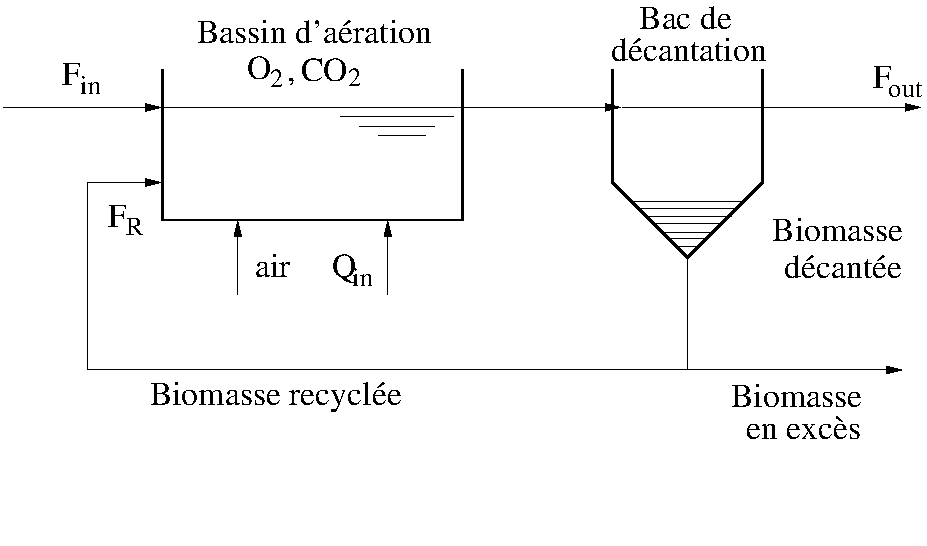
\includegraphics[width=11cm]{epurat} 
   \caption{Station d'épuration biologique aérobie}
   \label{Fig:epurat}
\end{figure}
Le bassin d'aération est alimenté par des eaux  usées
(débit
$F_{in}$) contenant un substrat organique polluant  (concentration $S$). 
Ce substrat organique est dégradé par des microorganismes
(concentration $X$) aérobies.  Cette dégradation nécessite de
l'oxygène dissous dans l'eau (concentration $O$) et produit du dioxyde
de carbone (concentration
$C$) sous forme dissoute mais qui se gazéifie aisément et sort du
système sous forme gazeuse.  L'oxygène dissout est fourni par un
système d'aération (débit d'air $Q_{in}$).  On fait l'hypothèse que
les dynamiques de transfert entre phase gazeuse et phase liquide sont
négligeables (instantanées).

La sortie du bassin d'aération est connectée à un bac de
sédimentation (décantation) où la biomasse (c'est à dire la masse 
des microorganismes) est séparée du reste.  L'eau clarifiée est
évacuée du système (débit $F_{out}$).  La biomasse est recyclée
vers le bassin d'aération (débit $F_R$).  Cependant, on prévoit la
possibilité d'éliminer la biomasse en excès (débit $F_S$).  Les
niveaux dans le bassin d'aération et dans le décanteur sont
supposés constants.  Le bassin d'aération est supposé parfaitement
mélangé.  Le bassin de décantation (qui ne peut être
parfaitement mélangé !) est modélisé par deux réservoirs
(compartiments) parfaitement mélangés (un pour l'eau clarifiée, un
pour la biomasse décantée).  On suppose aussi qu'il n'y a aucune
réaction biologique dans le décanteur. On demande d'établir un modèle d'état du système. \qed
\end{exercice}
\vv

\begin{exercice}{\bf \em Un système non conservatif}

Soit le réseau réactionnel suivant~:
\begin{equation*} \begin{split} 
X_1   &\longrightarrow X_2 + X_3 \\
X_3 &\longrightarrow 2X_1 + X_4
\end{split} \end{equation*}
\begin{enumerate}
\item Etablir le modèle d'état d'un système réactionnel fermé
sous les hypothèses de modélisation suivantes : principe d'action des
masses pour la première réaction avec une vitesse d'ordre 2
par rapport à tous les réactifs, cinétique de Michaelis-Menten pour
la deuxième réaction avec inhibition hyperbolique par $X_2$.
\item Montrer que le système n'est pas conservatif. Donner une
justification physique.
\item Montrer qu'il suffit d'ajouter un réactif initial dans la première 
ou la deuxième réaction pour rendre le système conservatif. \qed
\end{enumerate}
\end{exercice}

\end{document}
  

